\documentclass{beamer}
\usepackage{setspace}
\usepackage{bm,color,float,epstopdf,amsthm,epstopdf}
\usepackage{multirow}
\usepackage{tikz}
\usepackage{eurosym}
\usetikzlibrary{arrows,automata,fit}
\newtheorem{result}{Result}
\renewcommand{\arraystretch}{1.5}
\begin{document}

\begin{frame}{International Finance}
   \begin{itemize}
       \item International finance is a large and rich topic
       \item Today, we're going to price currencies
       \item We're going to study a couple of practical examples
   \end{itemize}
\end{frame}

\begin{frame}{Exchange Rates}
    \begin{itemize}
        \item Currencies are like tacos
        \item I go to 3 Amigos and buy tacos, I go to Chase and buy pesos
        \item In both cases, I pay with dollars
        \item Let $E$ denote the price of foreign currency
        \item E.g. a peso sells for $E=\$.05$ 
    \end{itemize}
\end{frame}

\begin{frame}{Example 1}
    \begin{itemize}
        \item Two countries, domestic ($D$) and foreign ($F$)
        \item $r_{D}$ is the risk-free rate in $D$, $r_{F}$ in $F$
        \item $E_{0}$ is the spot price of $F$'s currency
        \item $K_{0}$ is the price of a forward on $F$'s currency
    \end{itemize}
\end{frame}

\begin{frame}{Example 1}
    \begin{enumerate}
        \item Borrow $\$_{D}1$m in $D$
        \item Buy $\$_{D}1\text{m}/E_{0}$ of $F$'s currency (in $\$_{F}$)
        \item Buy $\$_{D}1\text{m}/E_{0}$ of $F$'s risk-free 
        \item Sell a forward in $F$ with price $K_{0}$ (in $\$_{D}$)
    \end{enumerate}
\end{frame}

\begin{frame}{Example 1}
    \begin{enumerate}\addtocounter{enumi}{4}
        \item In one year, we get  
            \begin{equation}
                (1+r_{F})\cdot (\$_{D}1\text{m}/E_{0})
            \end{equation}
            in $\$_{F}$
        \item We sell our $F$ currency for $K_{0}$ and get
            \begin{equation}
                K_{0}\cdot(1+r_{F})\cdot(\$_{D}1\text{m}/E_{0})
            \end{equation}
            in $\$_{D}$
        \item We repay our loan
            \begin{equation}
                K_{0}\cdot(1+r_{F})\cdot(\$_{D}1\text{m}/E_{0})-(1+r_{D})\cdot\$_{D}1\text{m}
            \end{equation}
            in $\$_{D}$
    \end{enumerate}
\end{frame}

\begin{frame}{Example 1}   
    \begin{itemize}
        \item You should \underline{not} be able to make money from this trade
        \item It requires no money down
        \item We conclude that
            \begin{equation}
                1+r_{D}\overset{\text{``should''}}{=}(1+r_{F})\cdot\frac{K_{0}}{E_{0}}
            \end{equation}
        \item\textbf{Warning:} the forward price on a $D$ asset is $K_{0}=S_{0}(1+r_{D})$. $F$'s currency is \underline{not} a $D$ asset (it has its own rate $r_{F}$). The forward price on an $F$ asset is its own thing. 
    \end{itemize}
\end{frame}

\begin{frame}{Board Problem 1}
        Suppose that
        \begin{enumerate}
            \item the risk-free rate is $r_{D}=5\%$ in the US 
            \item a euro sells for $E_{0}=\$.05$
            \item the forward price on pesos is 
        \end{enumerate}
        What should the risk-free rate be in the EU? What arbitrage opportunity is available to you if the risk-free rate in the EU is $r_{F}=10\%$? 
\end{frame}

\begin{frame}{Example 2}
    \begin{itemize}
        \item A taco in the US sells for USD\$3
        \item A taco in Mexico sells for MEX\$20
        \item A peso sells for \$.05.
        \item What arbitrage opportunity is available to you?
    \end{itemize}
    \begin{enumerate}
        \item Buy MEX\$20 for USD\$1
        \item Buy 1 taco in Mexico for MEX\$20
        \item Sell 1 taco in the US for USD\$3
        \item You've made USD\$2
    \end{enumerate}
\end{frame}

\begin{frame}{The Economist's Big-Mac Index}
    \begin{center}
        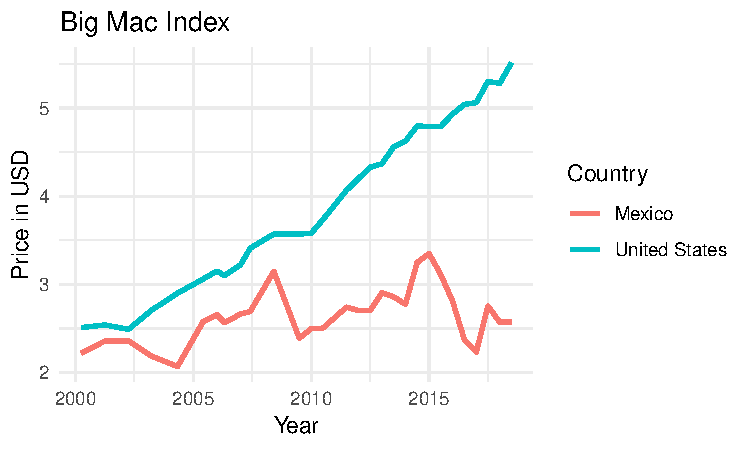
\includegraphics[scale=.75]{bigmac}
    \end{center}
    $\dagger$Courtesy of The Economist. 
\end{frame}

\begin{frame}
    \begin{center}
        {\Large\textbf{Last Deck! Woohoo!}}
    \end{center}
\end{frame}

\end{document}
